\documentclass[10pt,a4paper]{article}
\usepackage[utf8]{vietnam}
\usepackage{amsmath}
\usepackage{amsthm}
\usepackage{amsfonts}
\usepackage{amssymb}
\usepackage{graphicx}
\usepackage{mathrsfs}
\usepackage{url}
\usepackage{hyperref}
\usepackage{indentfirst}
\usepackage[section]{placeins}
\newtheorem{remark}{Nhận xét}
\author{Leopard Bethemel}
\title{Phân tích mức độ tương tác của người dùng\\đối với bài dịch Reddit trên RedditVN}
\date{\today}
\begin{document}
\maketitle
\renewcommand{\contentsname}{Mục lục}
\tableofcontents
\begin{abstract}
    \href{https://www.facebook.com/groups/redditvietnam/}{RedditVN} là phiên bản Việt Nam trên Facebook của \href{https://www.reddit.com/}{Reddit}. Các thành viên trong nhóm sẽ đóng góp các bài dịch từ những chủ đề trên Subreddit. Bản báo cáo này sẽ phân tích mức độ hưởng ứng của độc giả đối với bài dịch.

    \textbf{Chú ý:} Tác giả không khuyến khích các bạn chạy dịch giả theo số tương tác mà bỏ bê chất lượng dịch thuật. Đồng thời cũng không coi thường việc dịch theo sở thích hay cảm hứng. Tác giả chỉ muốn phần nào xem xét hiện tượng "flop" và giúp các bạn có biện pháp để giảm thiểu khả năng bị chìm.
\end{abstract}

\clearpage
\section{Thu thập dữ liệu}
Dữ liệu được cung cấp ở đây:

\href{https://mega.nz/#F!GMlQnKqZ!8FTQYeh8aprKPNE1qQT3ng}{https://mega.nz/\#F!GMlQnKqZ!8FTQYeh8aprKPNE1qQT3ng}

Trong thư mục \texttt{redditStats}, file \texttt{20170101T000000-20190101T000000.csv} chứa toàn bộ bài viết trong group RedditVN từ khi thành lập đến cuối năm 2018. Các bài đăng sau mốc trên vẫn còn tương tác ít nhiều, sẽ ảnh hưởng đến phân tích nói chung. Do đó, chúng ta chỉ tập trung vào khoảng thời gian trước năm 2019.

Ngoài ra, trước khi tool trợ giúp dịch thuật ra đời, bài dịch trong nhóm nói chung không theo một format thống nhất, dẫn đến không ít post không dẫn kèm link gốc. Hoặc hy hữu một số link gốc bị xóa hay khóa.

Sau khi loại bỏ các bài không thể truy ra ID Reddit hoặc có ID hỏng từ 28636 post, chúng ta còn 22869, chiếm 79,86\% tổng số. Mẫu dữ liệu này có thể coi là hợp lệ để nghiên cứu.

\section{Subreddit được dịch nhiều nhất}
\subsection{Trung bình}
Trong vòng hai năm qua (2017-2018), đã có 1417 subreddit khác nhau được dịch. Trung bình mỗi sub có 16,13 bài.
\begin{itemize}
    \item 783 sub (tức 55,26\%) có trên 1 bài viết.
    \item 226 sub (tức 15,95\%) có trên 10 bài viết.
    \item 38 sub (tức 2,46\%) có trên 100 bài viết.
\end{itemize}

\subsection{Tổng}
Chúng ta xem xét 30 subreddit được dịch nhiều nhất.
\begin{figure}[!h]
    \centering
    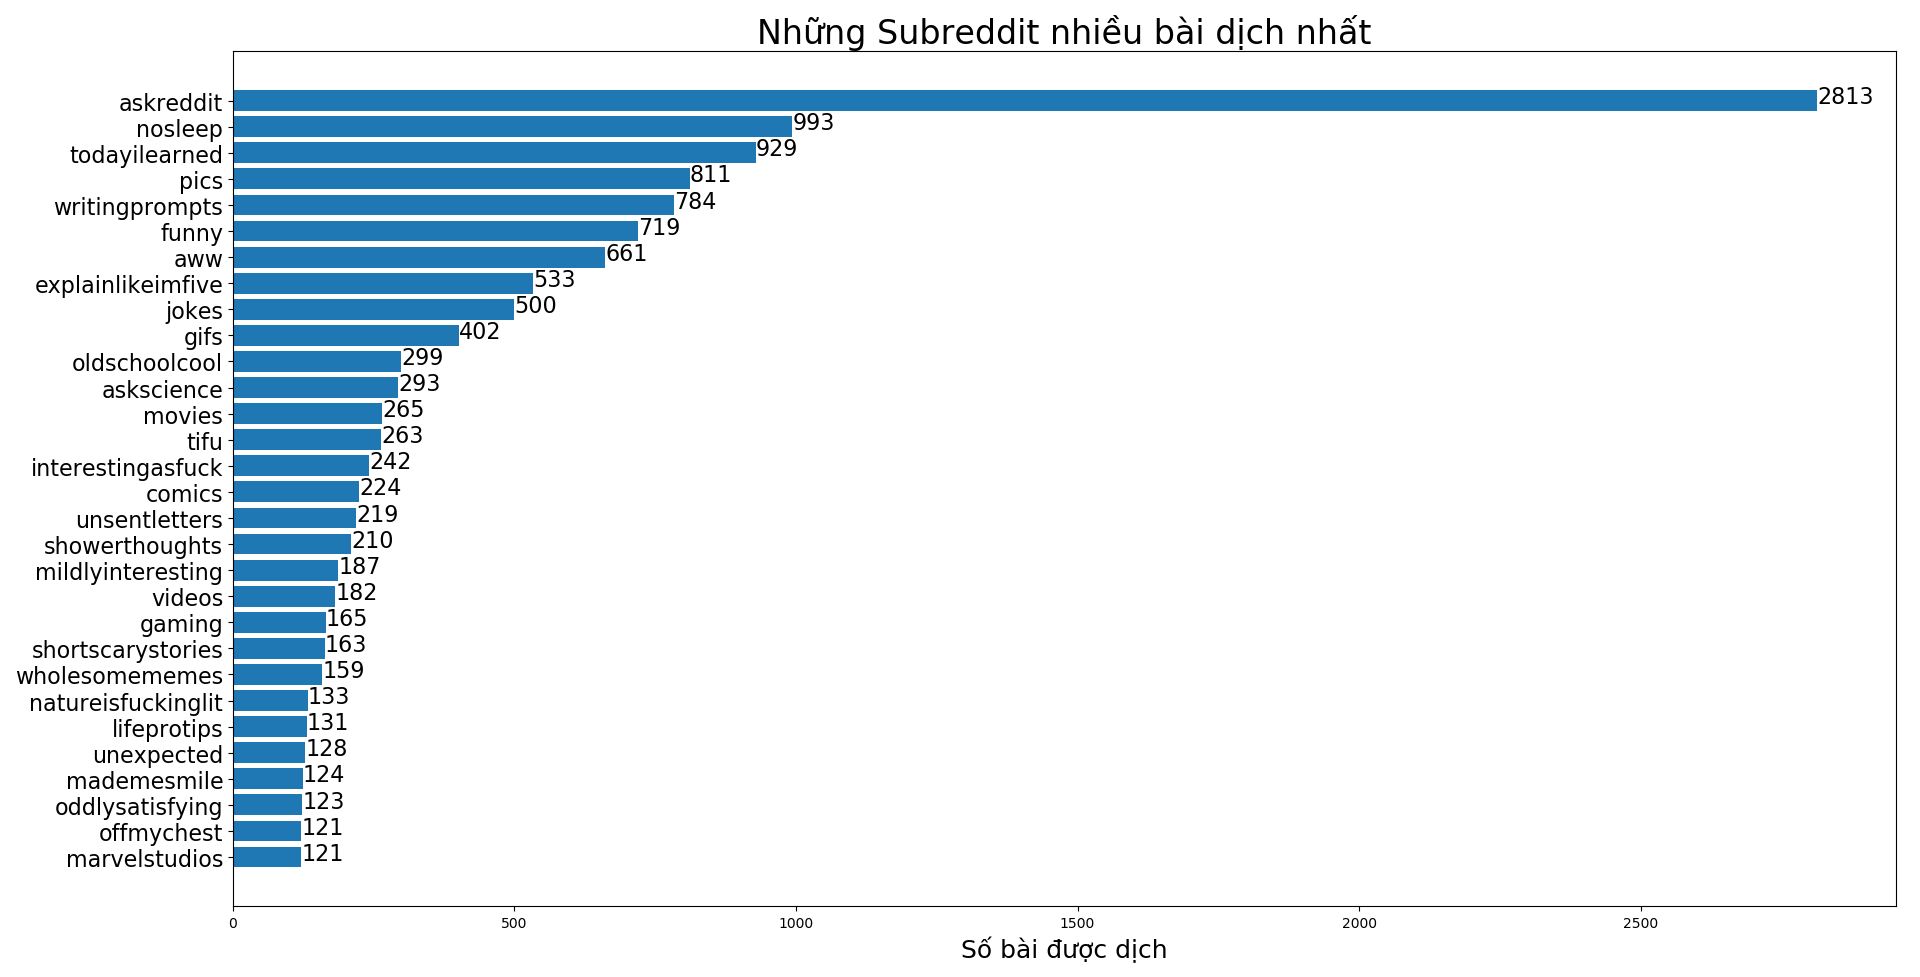
\includegraphics[width=\textwidth]{img/TopTranslatedSubreddits.png}
    \caption{30 Subreddit được dịch nhiều nhất}
    \label{fig:toptranslatedsubreddits}
\end{figure}

Dễ thấy chủ đề được các dịch giả RedditVN chọn nhiều nhất là \textbf{askreddit}, với xấp xỉ 2800 bài, nhiều gấp 2.5 lần so với \textbf{nosleep}, \textbf{todayilearned} đứng ở vị trí thứ thứ hai và ba. Các sub như \textbf{pics}, \textbf{writingprompts}, \textbf{funny} và \textbf{aww} cũng được dịch không ít, khoảng 660-810 bài cho mỗi sub. 23 subreddit còn lại có số bài viết phân bố trong khoảng [120, 480], nhưng một nửa là dưới 200 bài.

\begin{remark}
    \label{re:top6subreddits}
    Chúng ta hầu hết tập trung dịch vào 7 subreddit kể trên.
\end{remark}

\section{Subreddit được chú ý nhất}
\label{sec:interest}

Để tiện cho so sánh, chúng ta coi như comment và like có giá trị ngang nhau và sẽ đếm tổng của số lượt like (kể cả cảm xúc) và số comment.
\subsection{Tổng}
\begin{figure}[!h]
    \centering
    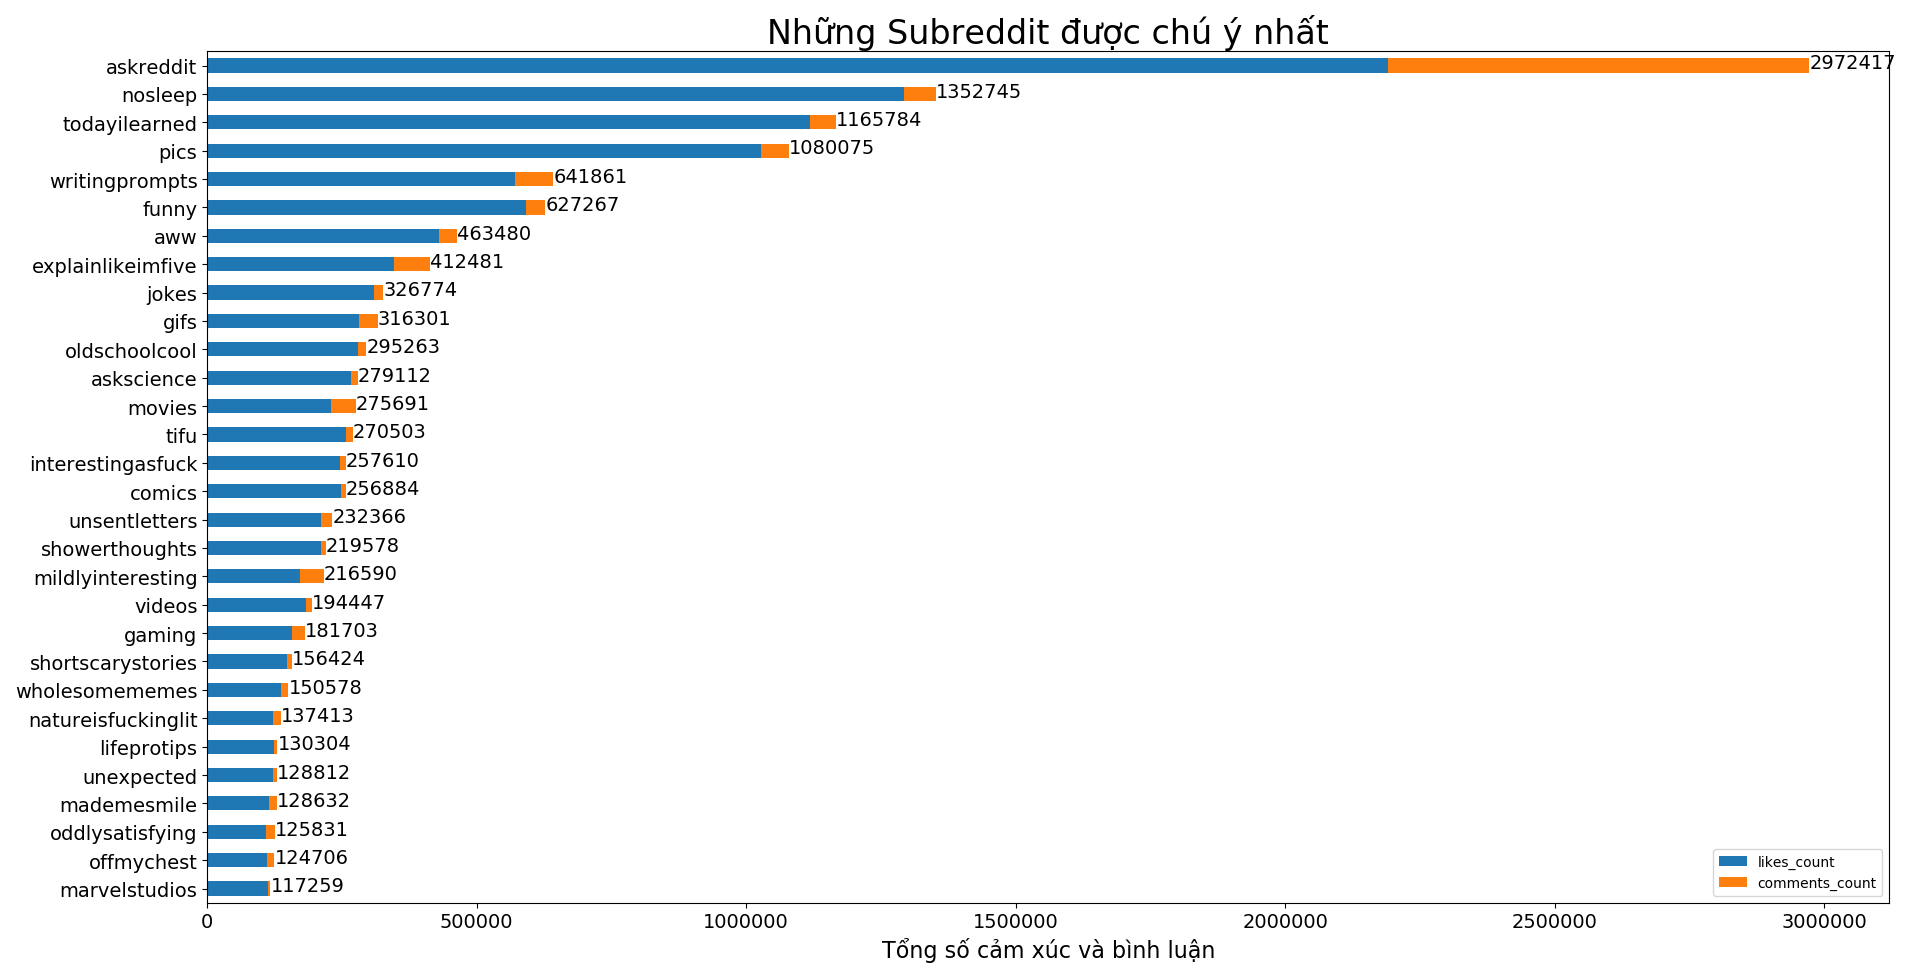
\includegraphics[width=\textwidth]{img/TopAttentionSubreddits.png}
    \caption{30 Subreddit được chú ý nhất}
    \label{fig:topattentionsubreddits}
\end{figure}

\textbf{askreddit} tiếp tục giữ vị trí độc tôn với tổng số lượt thích (cũng như cảm xúc khác) và bình luận cao chót vót gần 3 triệu, gấp đôi á quân \textbf{nosleep} quen thuộc. \textbf{todayilearned} và \textbf{pics} bám đuổi sát sao ở số 3 và số 4. Các vị trí tiếp theo, với tổng số like và comment dưới 650 nghìn, nhìn chung không khác mấy so với hình \eqref{fig:toptranslatedsubreddits}. Ta có thể kết luận rằng:
\begin{remark}
    \label{re:attentionandtranslation}
    \textbf{"Sub được dịch nhiều"} tương đương với \textbf{"bài sẽ nhiều tương tác"}.
\end{remark}

Một điều đặc biệt là \emph{tổng số comment} trong \textbf{askreddit} nhiều hơn hẳn so với các sub khác ít nhất 11 lần. Nói cách khác:
\begin{remark}
    \label{re:askredditpotential}
    \textbf{askreddit} có tiềm năng thu hút bình luận cao hơn các subreddit khác rõ rệt.
\end{remark}
\subsection{Trung bình}
So về trung bình (bảng \eqref{tab:meaninterests}), \textbf{askreddit} tuy thuộc top trong các sub "nhiều chữ" như \textbf{nosleep}, \textbf{todayilearned}, \textbf{tifu} nhưng thua xa các sub thiên về hình ảnh trực quan như \textbf{pics}, \textbf{aww}, \textbf{funny}, \textbf{gifs}. Do đó:
\begin{remark}
    \label{re:toomuchwords}
    Độc giả nhìn chung ngại đọc nhiều chữ.
\end{remark}

Một giải pháp khắc phục là sử dụng hình minh họa bắt mắt để kéo thêm tương tác. (Cần phải có thêm một nghiên cứu khác về mức độ tương tác và hình ảnh để xác định tính hiệu quả của phương pháp này)

\begin{table}[hp]
    \centering
    \begin{tabular}{|c|c|c|}
        \hline
        Subreddit & Số phản ứng trung bình & Số bình luận trung bình \\
        \hline
        \textbf{tổng thể} & \textbf{874} & \textbf{111} \\
        \hline
        askreddit & 779 & 278 \\
        \hline
        pics & 1595 & 73 \\
        \hline
        aww & 1693 & 71 \\
        \hline
        funny & 1429 & 73 \\
        \hline
        todayilearned & 614 & 76 \\
        \hline
        gifs & 1473 & 88 \\
        \hline
        jokes & 861 & 65 \\
        \hline
        nosleep & 349 & 66 \\
        \hline
        interestingasfuck & 1275 & 75 \\
        \hline
        writingprompts & 360 & 44 \\
        \hline
        comics & 1245 & 73 \\
        \hline
        wholesomememes & 1679 & 77 \\
        \hline
        explainlikeimfive & 431 & 86 \\
        \hline
        oldschoolcool & 861 & 44 \\
        \hline
        mildlyinteresting & 1314 & 64 \\
        \hline
        mademesmile & 2005 & 67 \\
        \hline
        videos & 1158 & 118 \\
        \hline
        oddlysatisfying & 1712 & 73 \\
        \hline
        movies & 650 & 168 \\
        \hline
        unexpected & 1431 & 88 \\
        \hline
        tifu & 595 & 96 \\
        \hline
        natureisfuckinglit & 1113 & 63 \\
        \hline
        blackpeopletwitter & 1461 & 140 \\
        \hline
        wtf & 1020 & 135 \\
        \hline
        beamazed & 1710 & 75 \\
        \hline
        memes & 1777 & 90 \\
        \hline
        natureismetal & 979 & 111 \\
        \hline
        showerthoughts & 520 & 79 \\
        \hline
        gaming & 677 & 79 \\
        \hline
        hmmm & 988 & 41 \\
        \hline
    \end{tabular} 
    \caption{Số phản ứng và bình luận trung bình của 30 sub nổi nhất và tổng thể}
    \label{tab:meaninterests}   
\end{table}

\section{Xu thế đăng bài theo thời gian}
Vì không có điều kiện gì khác, chúng ta sẽ giả sử rằng mọi bài viết trong dữ liệu đều được duyệt và các mod/admin không thiên vị khung giờ hay người đăng.

\subsection{Tổng quan}

Bài dịch đầu tiên được đăng vào 18:59:17+0700 ngày 28/04/2017. Từ khi thành lập (tháng 4 / 2017), số lượng bài viết và tương tác tăng dần, mặc dầu có giảm một chút vào giai đoạn đầu năm 2018. 
\begin{figure}[!h]
    \centering
    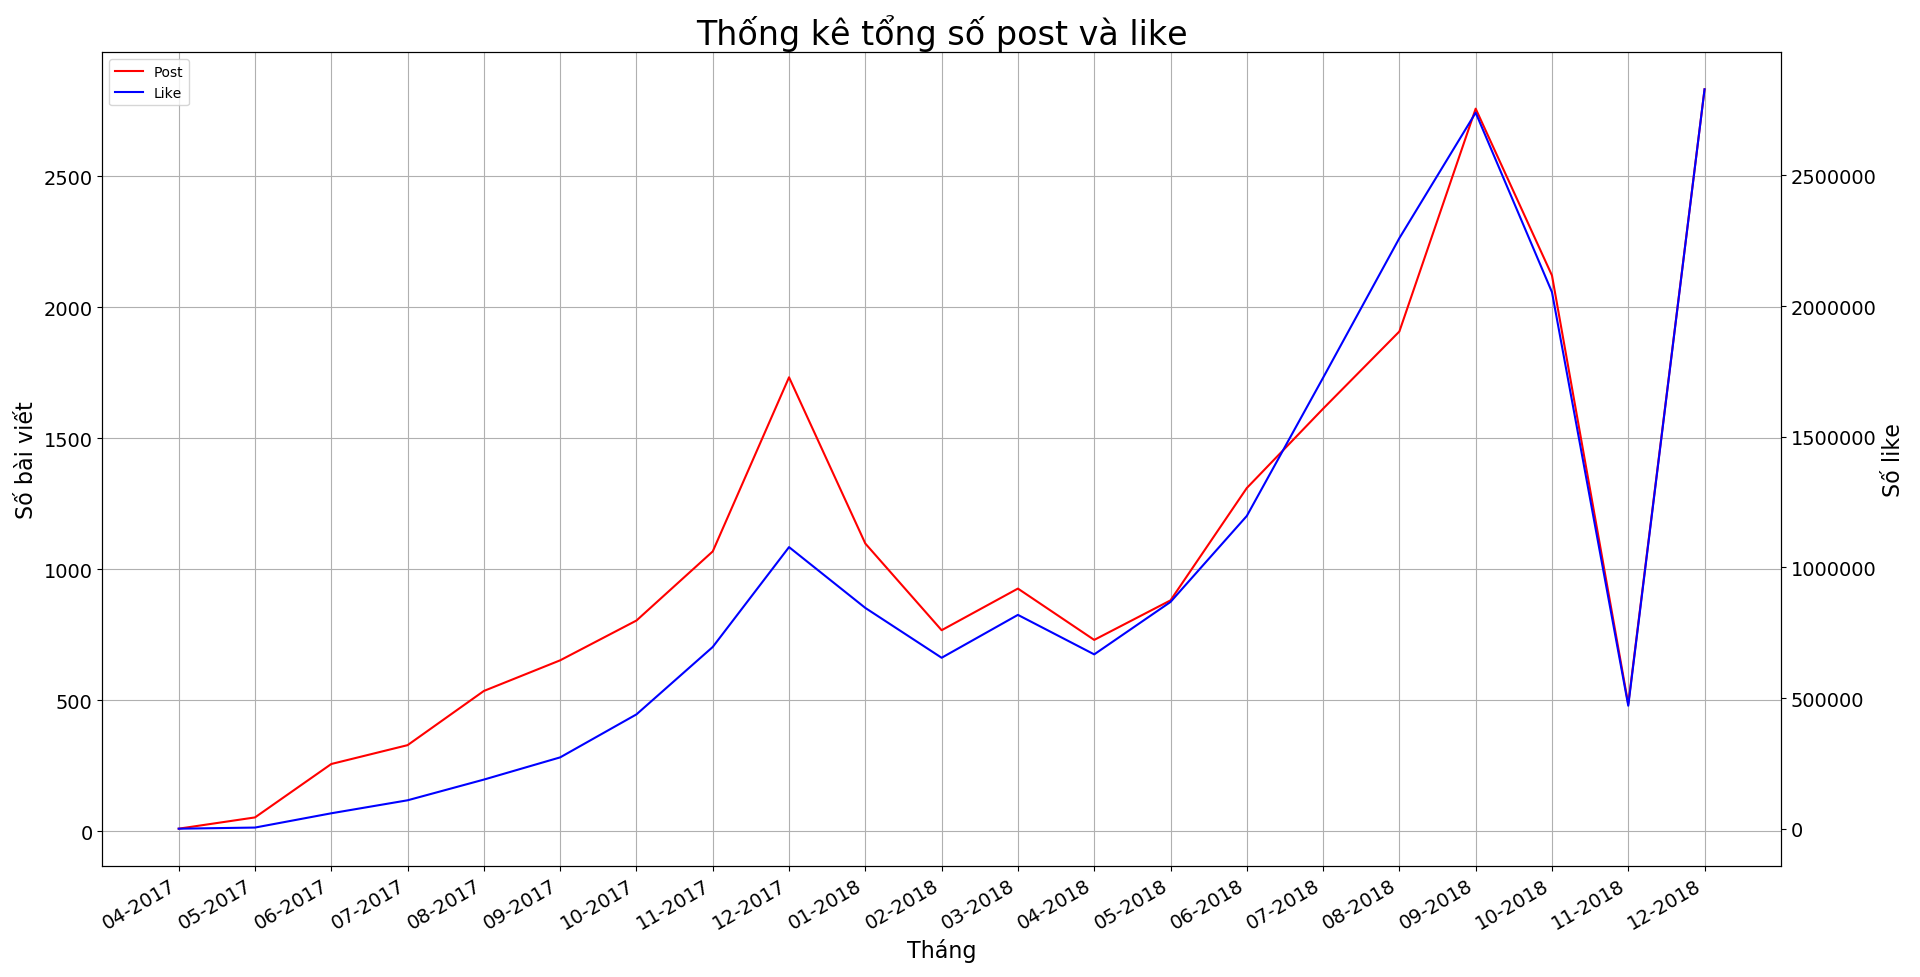
\includegraphics[width=\textwidth]{img/AllLikesPostsOverTime.png}
    \caption{Tổng số post và like qua từng tháng}
    \label{fig:alllikespostsovertime}
\end{figure}

Tuy nhiên, đến tháng 10 và 11 cùng năm, từ vị trí cao nhất biểu đồ tính tới thời điểm ấy (khoảng 2800 post và 2800000 like), số bài viết và tương tác rớt dốc thê thảm xuống còn 1/5. Nguyên nhân vẫn chưa được xác định, song có thể phỏng đoán là do cuộc "Đại Thanh Trừng" khiến số lượng thành viên sụt giảm nghiêm trọng. (Cần kiểm chứng). May mắn thay, tháng tiếp theo, con số đã phục hồi và còn nhỉnh hơn lúc trước.

\subsection{Mỗi tháng của từng sub}
Chúng ta sẽ quan sát số lượng post của 15 chủ đề được dịch nhiều nhất từ tháng 4/2017 đến tháng 12/2018.

\begin{figure}[h]
    \centering
    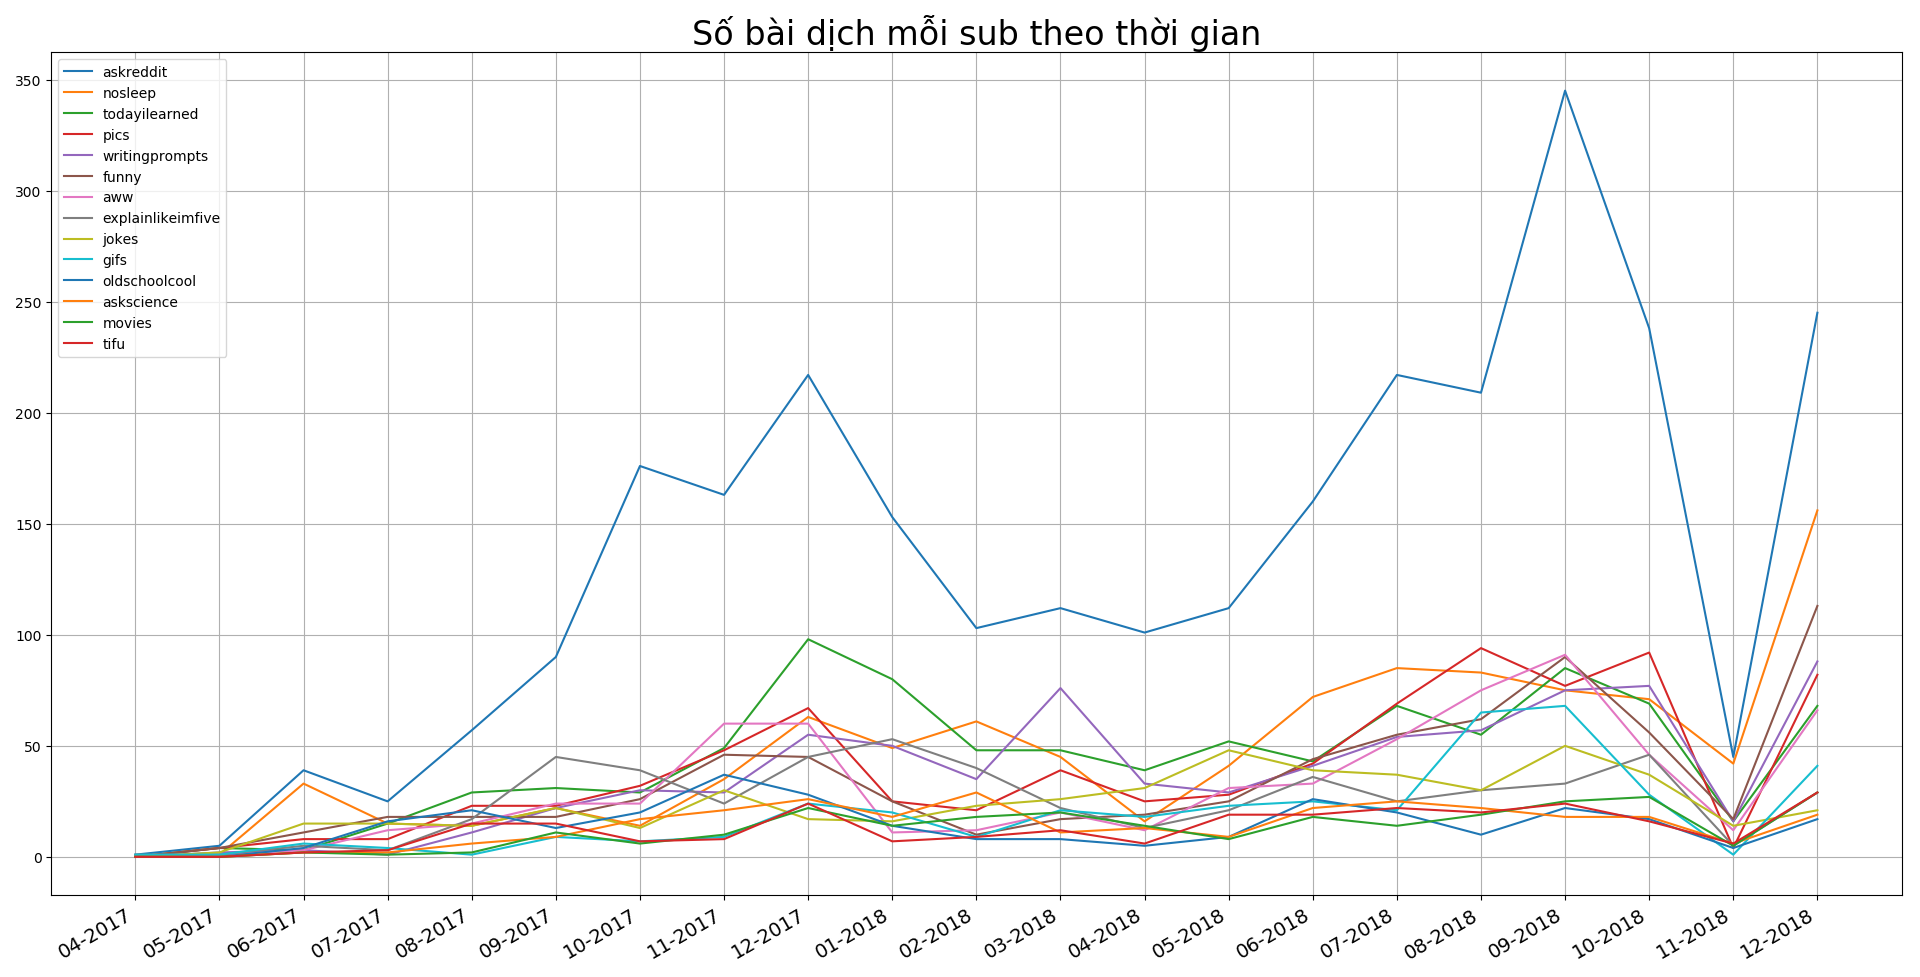
\includegraphics[width=\textwidth]{img/PostsOverTime.png}
    \caption{Số lượng bài viết của 15 sub được dịch nhiều nhất, chia theo từng tháng}
    \label{fig:postsovertime}
\end{figure}

Tuy số lượng tăng giảm không đều nhưng có thể thấy \textbf{askreddit} luôn chiếm vị trí số 1 trong danh sách những sub được chọn để dịch. Nhờ vào nhận xét \eqref{re:attentionandtranslation}, ta có thể suy ra \textbf{askreddit} sẽ nhận được lượng tương tác cực kỳ lớn.

\subsection{Theo khung giờ}
\subsubsection{Tổng thể}
\begin{figure}[ht]
    \centering
    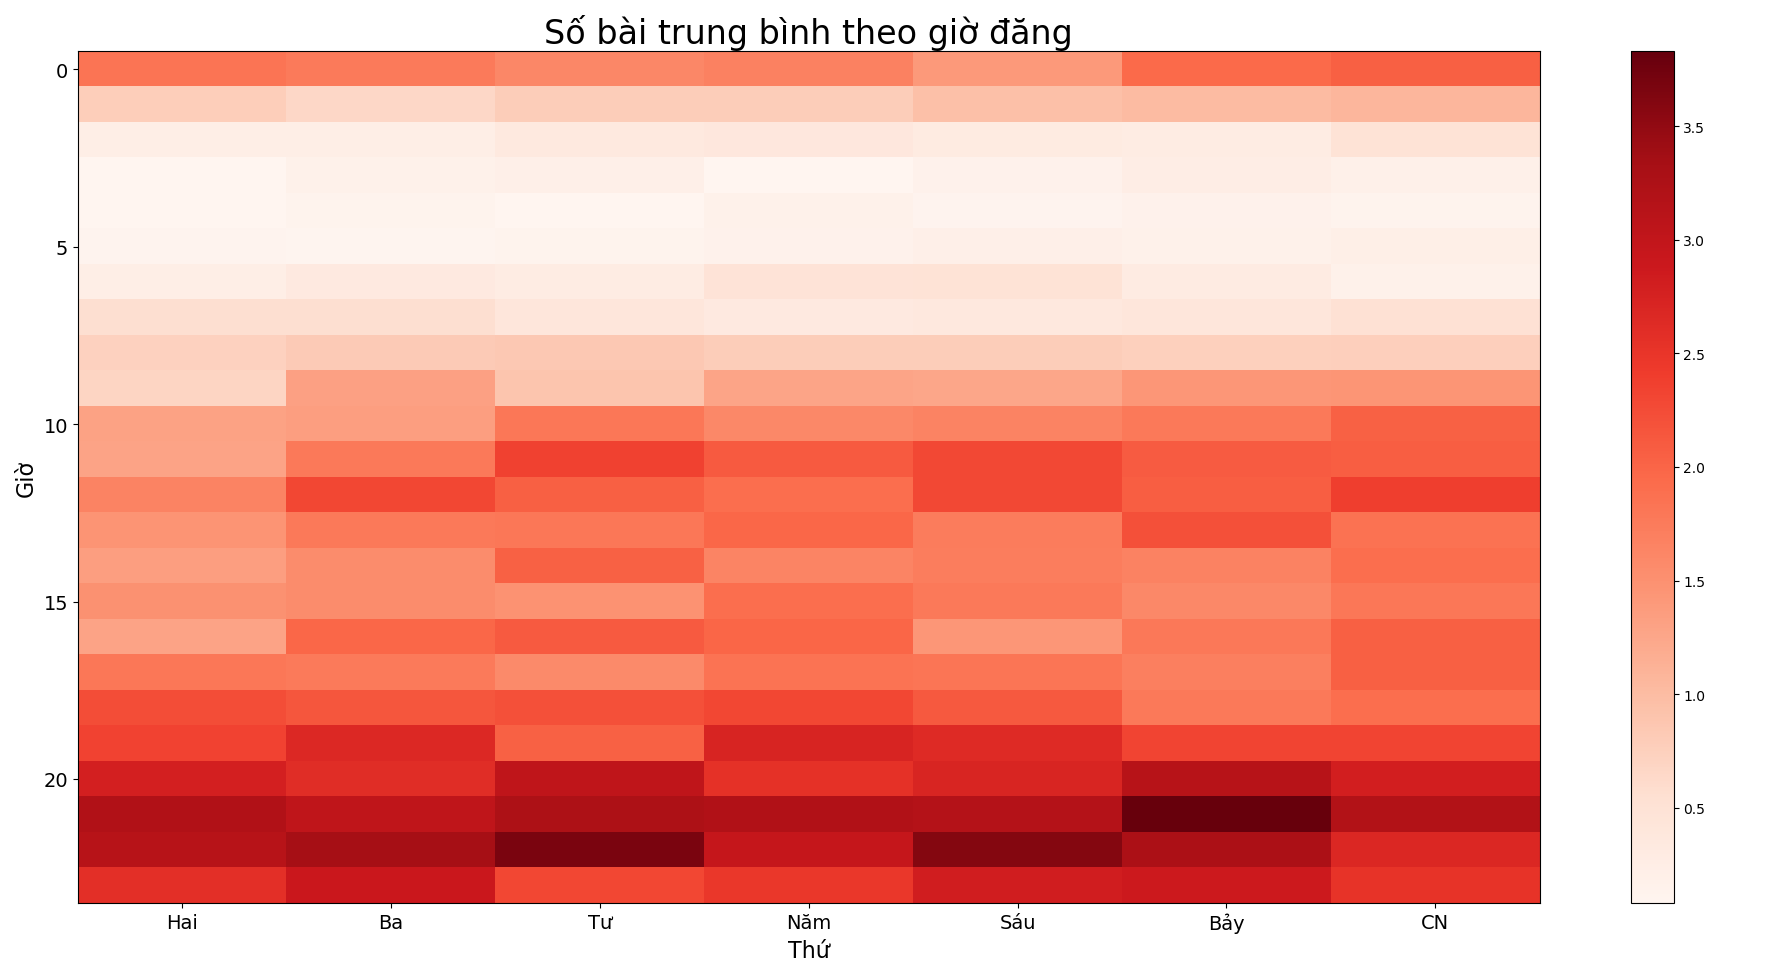
\includegraphics[width=0.9\textwidth]{img/MeanPostsWeekdayHour.png}
    \caption{Tần số post bài theo giờ tổng thể}
    \label{fig:meanpostsweekdayhour}
\end{figure}

Dựa vào dải màu đậm dưới cùng (hình \eqref{fig:meanpostsweekdayhour}), chúng ta suy ra dịch giả có thói quen đăng bài nhiều vào chiều và đặt biệt là giờ tối sau 20 giờ cho tới nửa đêm. Cảnh tượng chen chúc giành sự chú ý của người đọc ắt hẳn không tránh khỏi.

Trái lại, khoảng 1 giờ tới 8 giờ lại vắng tanh. Bài post vào giai đoạn này hứa hẹn sẽ bớt tranh chấp hơn.
\subsubsection{Chi tiết}
\begin{figure}[ht]
    \centering
    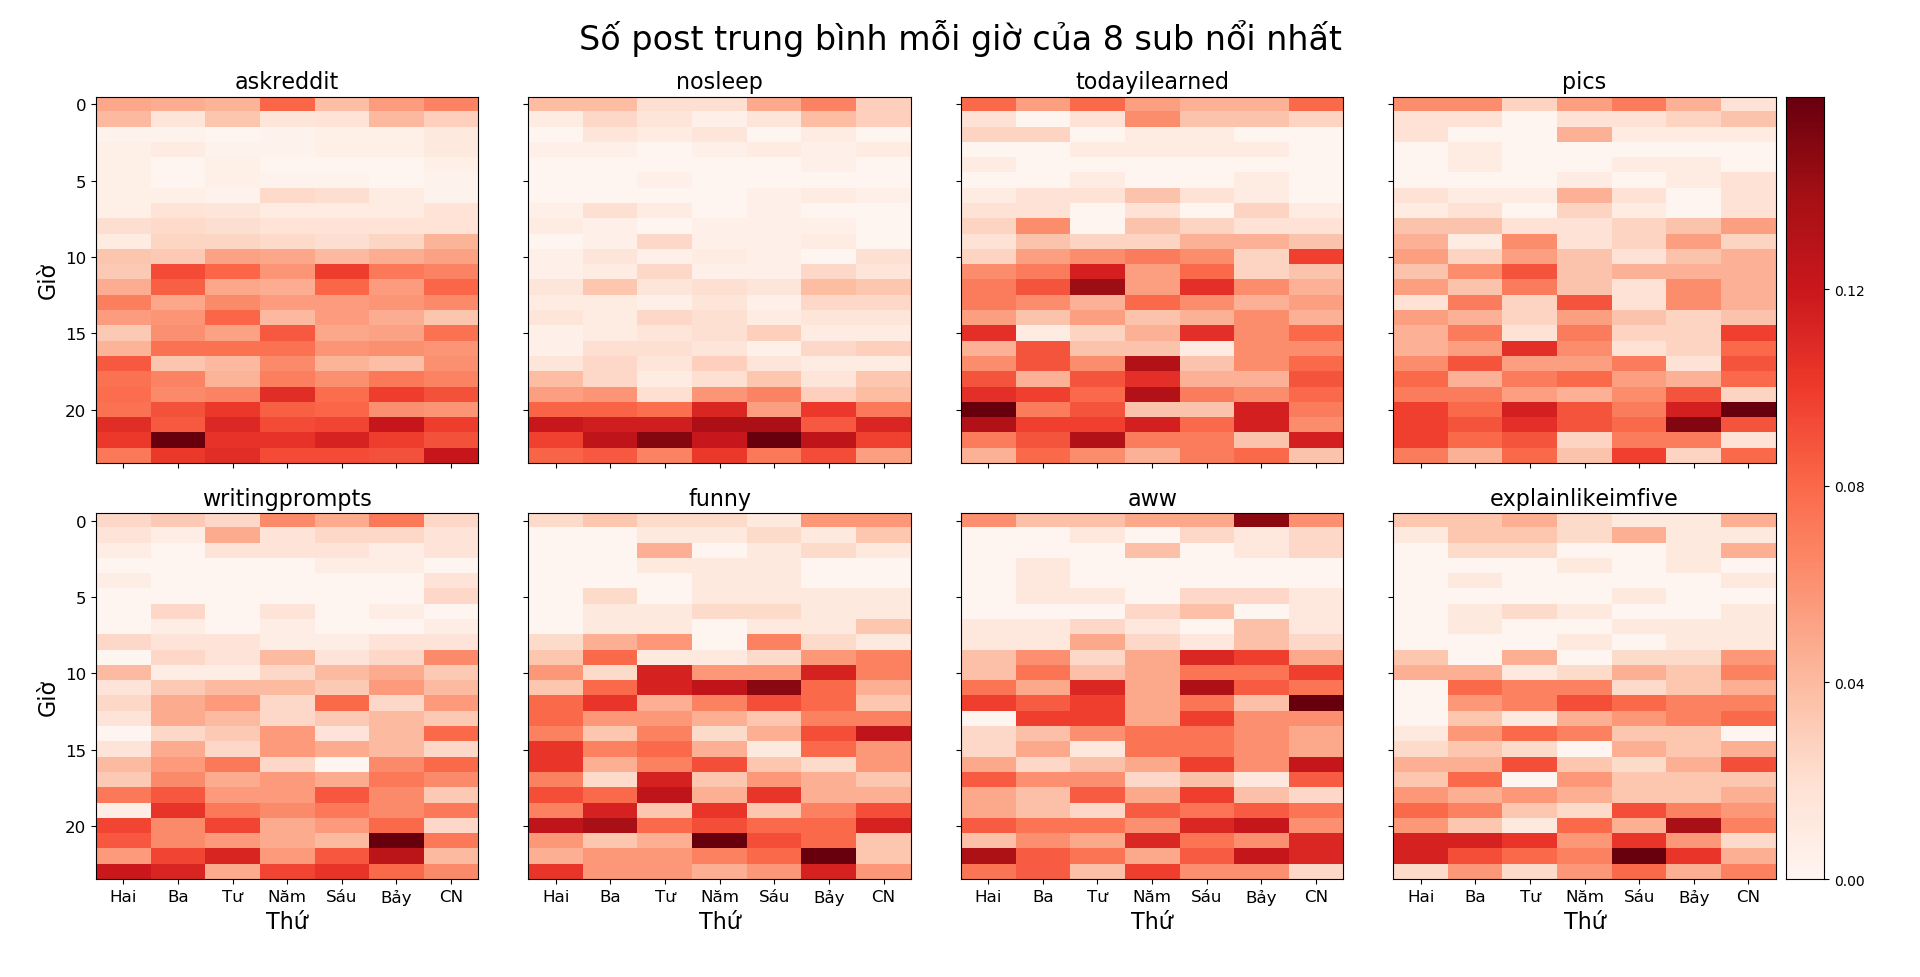
\includegraphics[width=\textwidth]{img/MeanPostsWeekdayHourPerSub.png}
    \caption{Tần số post bài theo giờ của 8 sub nổi nhất}
    \label{fig:meanpostsweekdayhourpersub}
\end{figure}

Các sub nổi nhất nói chung đều tuân theo quy luật của tổng thể, ngoại trừ \textbf{nosleep} hay xuất hiện vào giờ ngủ nghỉ 21 tới 24 giờ. Điều này khá dễ hiểu bởi tính chất ma quỷ hù dọa của \textbf{nosleep}, người dịch sẽ không muốn nhát ma người khác vào ban ngày ban mặt.

Ngoài ra, các sub khác đều tuân theo quy luật tổng thể. Nhưng chỉ có \textbf{askreddit} là đăng khá đồng đều giữa các khung giờ.

\section{Mức độ tương tác}
Một khi đã biết xu hướng đăng bài của dịch giả, hãy cùng xem độc giả hưởng ứng thế nào.

Từ phần \eqref{sec:interest}, chúng ta thấy rằng số lượng comment so với số like là không đáng kể, trừ \textbf{askreddit}. Vì vậy, để xem xét xu hướng phản ứng, chúng ta chỉ nên tính số lượng like. Chú ý: Dữ liệu like sẽ bao gồm mọi cảm xúc khác như phẫn nộ, haha, v.v.

\subsection{Thống kê tổng quát}
Tổng số like: 19976881.

Số like trung bình mỗi post: 873.54

Số like cao nhất: 9481

Bài nhiều like nhất: 

\href{https://www.facebook.com/groups/redditvietnam/permalink/710564989340906/}{https://www.facebook.com/groups/redditvietnam/permalink/\\710564989340906/}

\begin{itemize}
    \item 20408 bài (89,24\%) đạt 100 like trở lên.
    \item 15463 bài (67,62\%) đạt 300 like trở lên.
    \item 12188 bài (53,29\%) đạt 500 like trở lên.
    \item 6981 bài (30,53\%) đạt 1000 like trở lên.
    \item 2555 bài (11,17\%) đạt 2000 like trở lên.
    \item 305 bài (1,33\%) đạt 4000 like trở lên.
    \item 29 bài (0,13\%) đạt 6000 like trở lên.
    \item 2 bài (0,01\%) đạt 8000 like trở lên.
\end{itemize}

\begin{figure}[!ht]
    \centering
    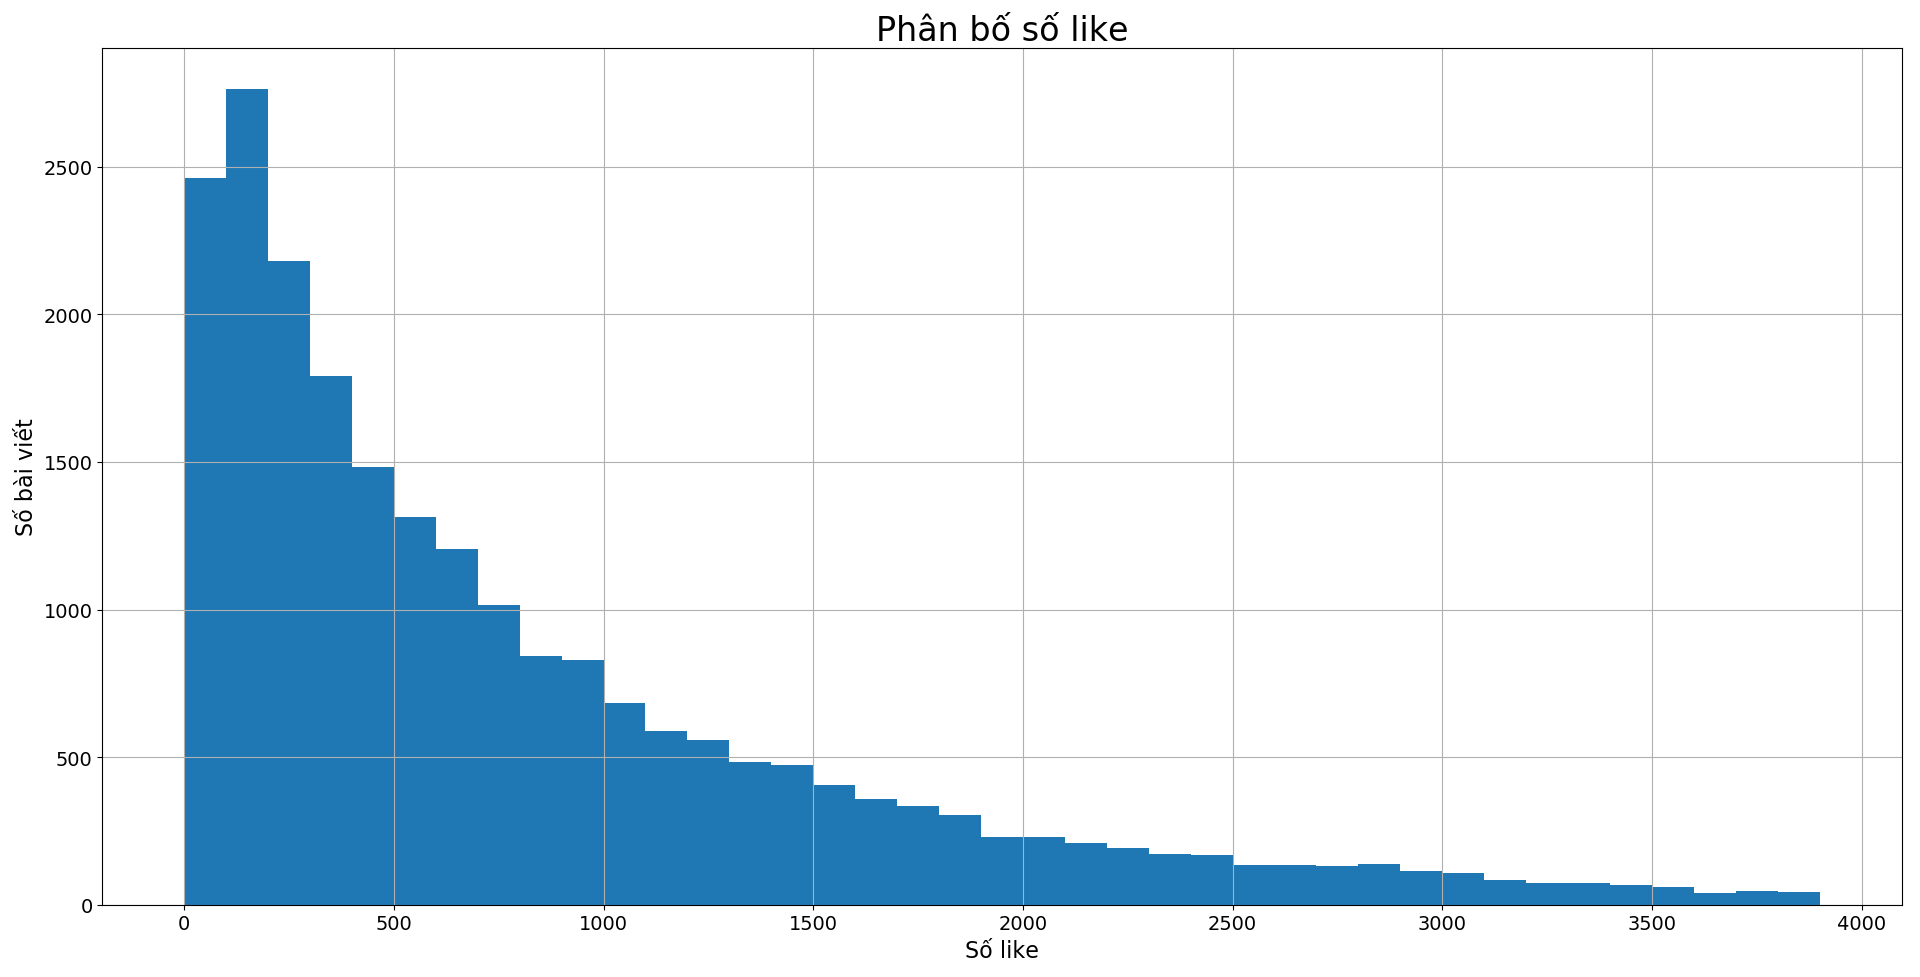
\includegraphics[width=\textwidth]{img/LikesDistribution.png}
    \caption{Phân bố like}
    \label{fig:likesdistribution}
\end{figure}

Có ít hơn 5\% số bài viết đạt 4000 like trở lên, nên để khảo sát mật độ tập trung của like, chúng ta chỉ cần chú ý vào những bài viết 4000 like trở xuống.

\begin{figure}[!h]
    \centering
    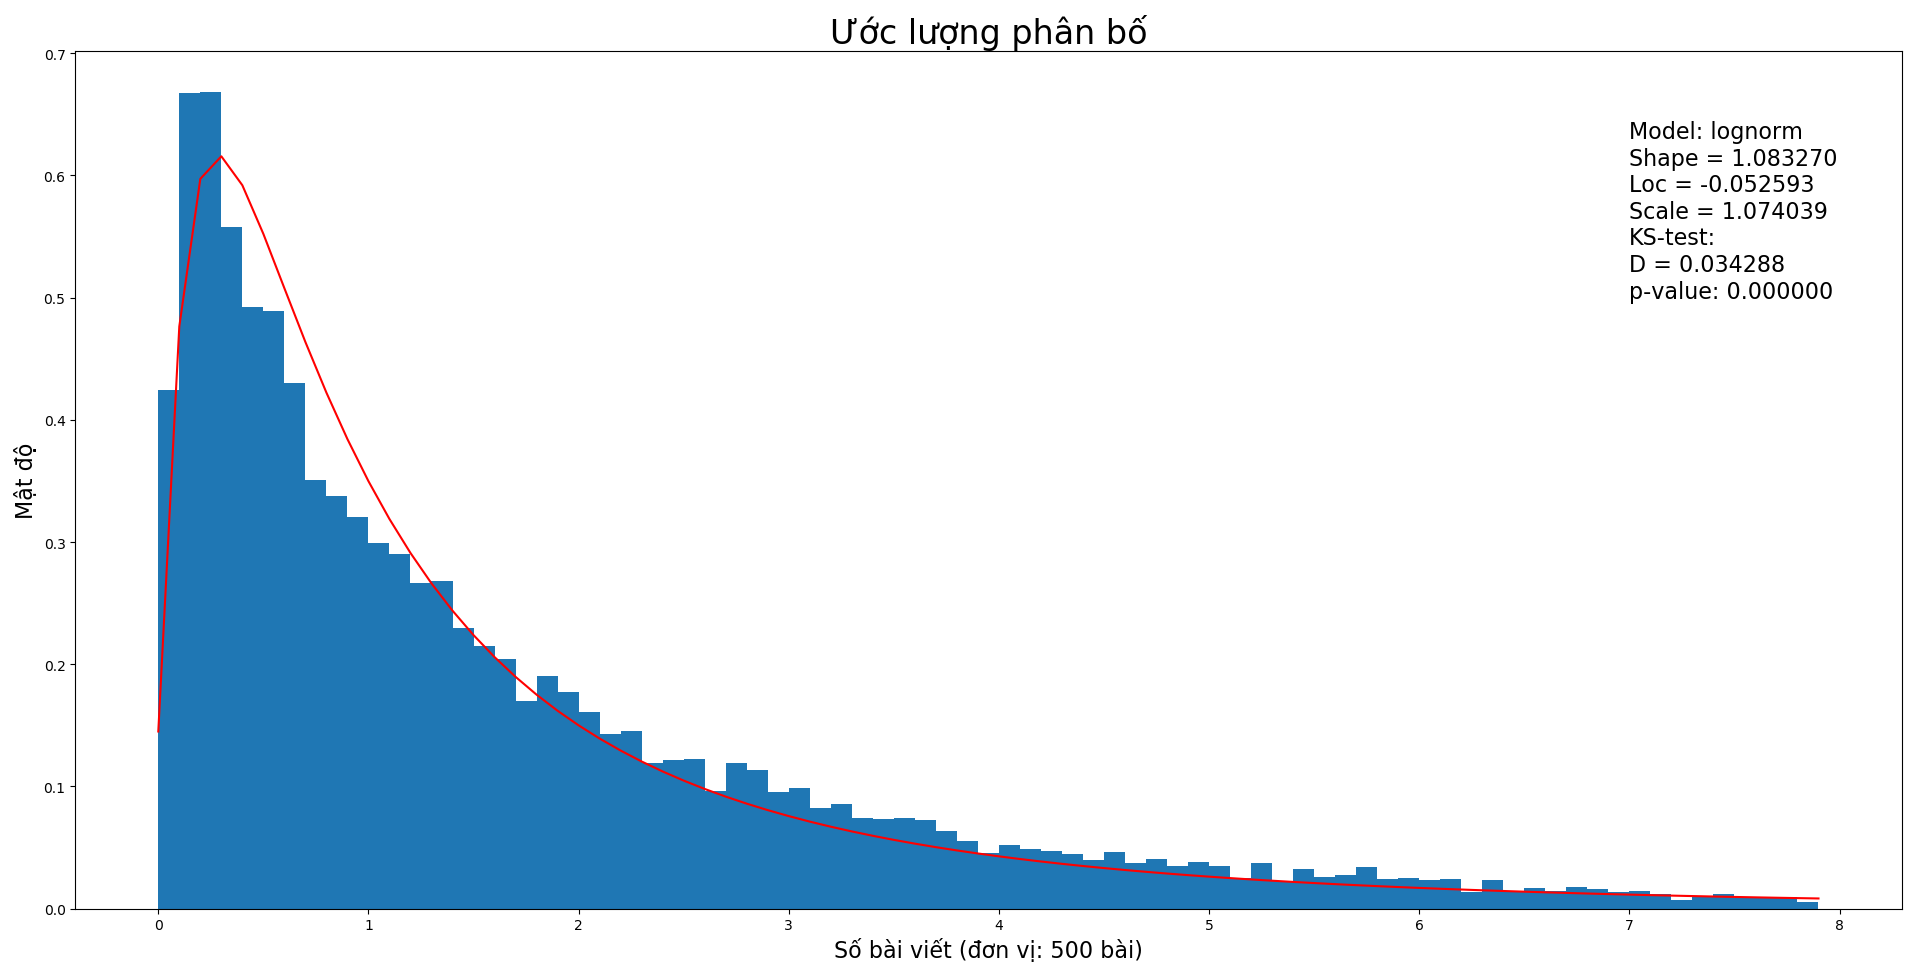
\includegraphics[width=\textwidth]{img/FitLikesDistribution.png}
    \caption{Mô hình phân bố like}
    \label{fig:fitlikesdistribution}
\end{figure}
Dễ thấy thông thường like tập trung ở 100-200 rồi giảm dần. Mô hình hóa phân bố này cho ta nhiều lựa chọn ban đầu: exponential, gamma, lognormal. Kết hợp với test Kolmogorov-Smirnov, chúng ta thấy exponential và lognormal là hợp nhất. Mặt khác, exponential không tạo ra một "đỉnh" núi ở giữa phân bố như lognormal. Cho nên chúng ta sẽ chọn mô hình lognormal với $p-value = 8.85521235143507 \times 10^{-24} < 1\%$, bất chấp $p-value$ của exponential nhỏ hơn.

\subsection{Theo giờ đăng}
\subsubsection{Tổng thể}
Ô màu trên sơ đồ \eqref{fig:meanlikesweekdayhour} càng đậm thì càng được nhiều like. Nhìn tổng quan, hầu hết sơ đồ có màu đỏ vừa ở mức 600 like trở lên, tức là group RedditVN có lượng tương tác lớn.
\begin{figure}[!ht]
    \centering
    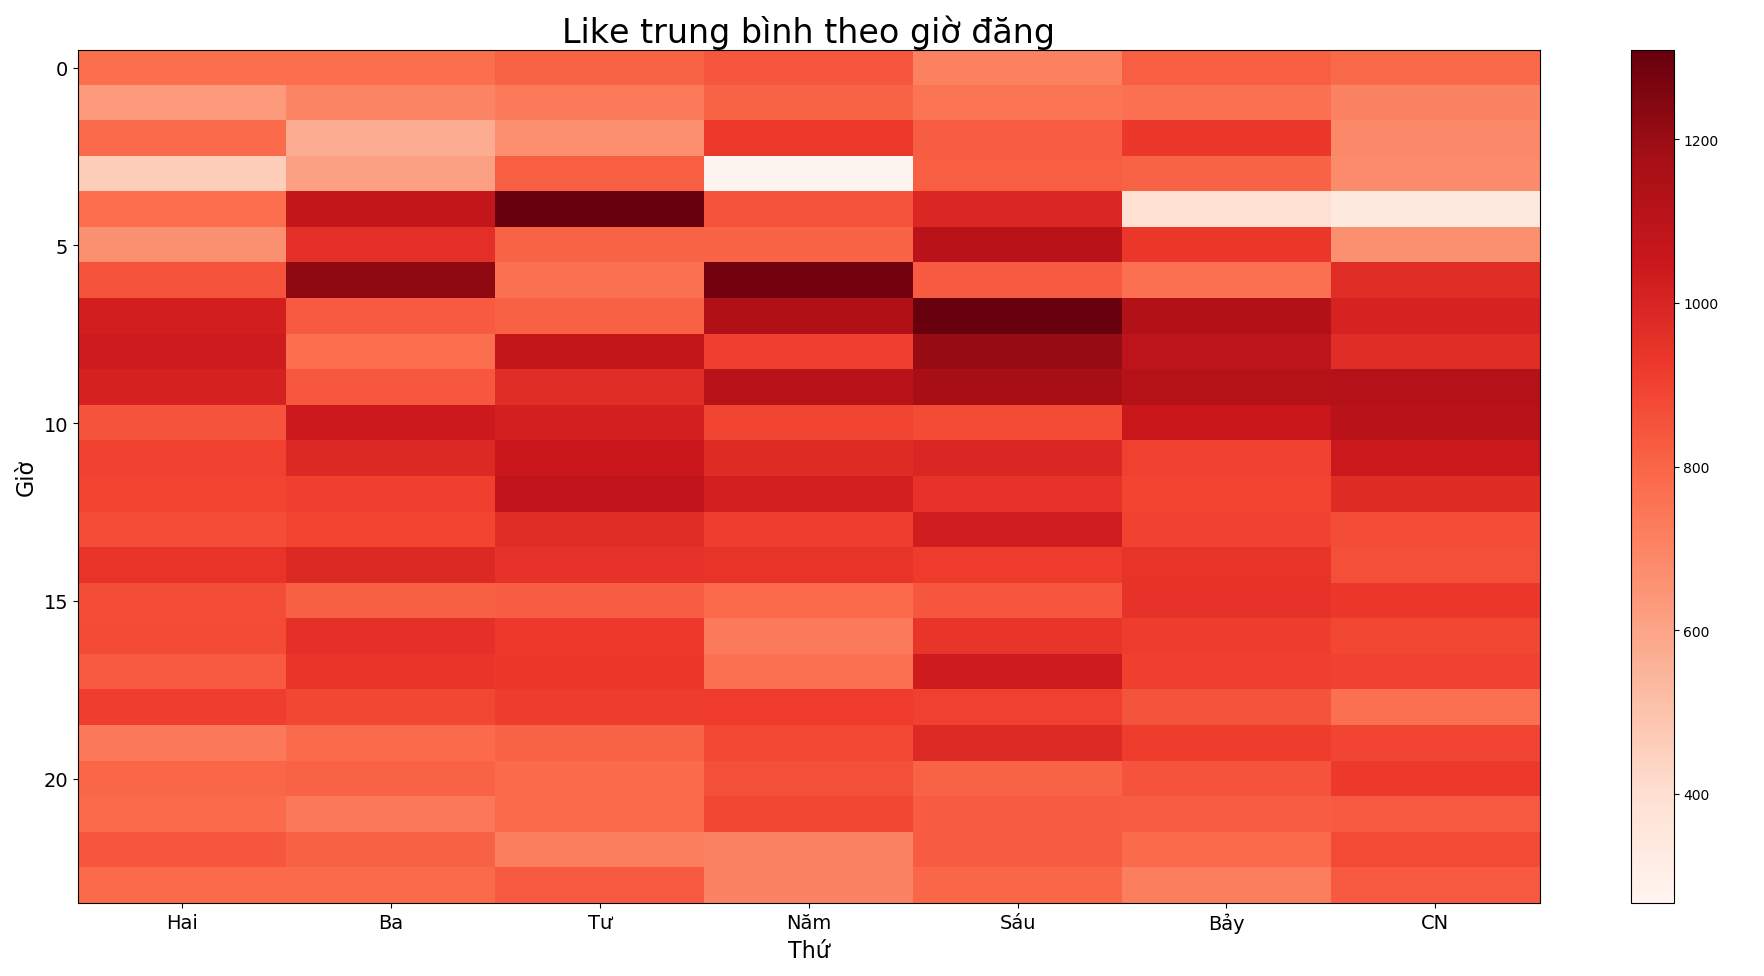
\includegraphics[width=\textwidth]{img/MeanLikesWeekdayHour.png}
    \caption{Like trung bình của post tính theo giờ đăng}
    \label{fig:meanlikesweekdayhour}
\end{figure}

Trái ngược với xu hướng đăng bài, các bài đăng vào khoảng 4 đến 10 giờ sáng nhìn chung được độc giả tương tác đáng kể. Những post buổi chiều và tối thì ít dần và thấp nhất là khuya tới sáng sớm 3 giờ.

\begin{remark}
    \label{re:time}
    Nên dàn xếp đăng bài vào giờ sáng để tránh chen chân nhau.
\end{remark}
\subsubsection{Đối với các sub nổi nhất}
Chúng ta sẽ tiếp tục mổ xẻ mức tương tác đối với từng sub nổi nhất.
\begin{figure}[!h]
    \centering
    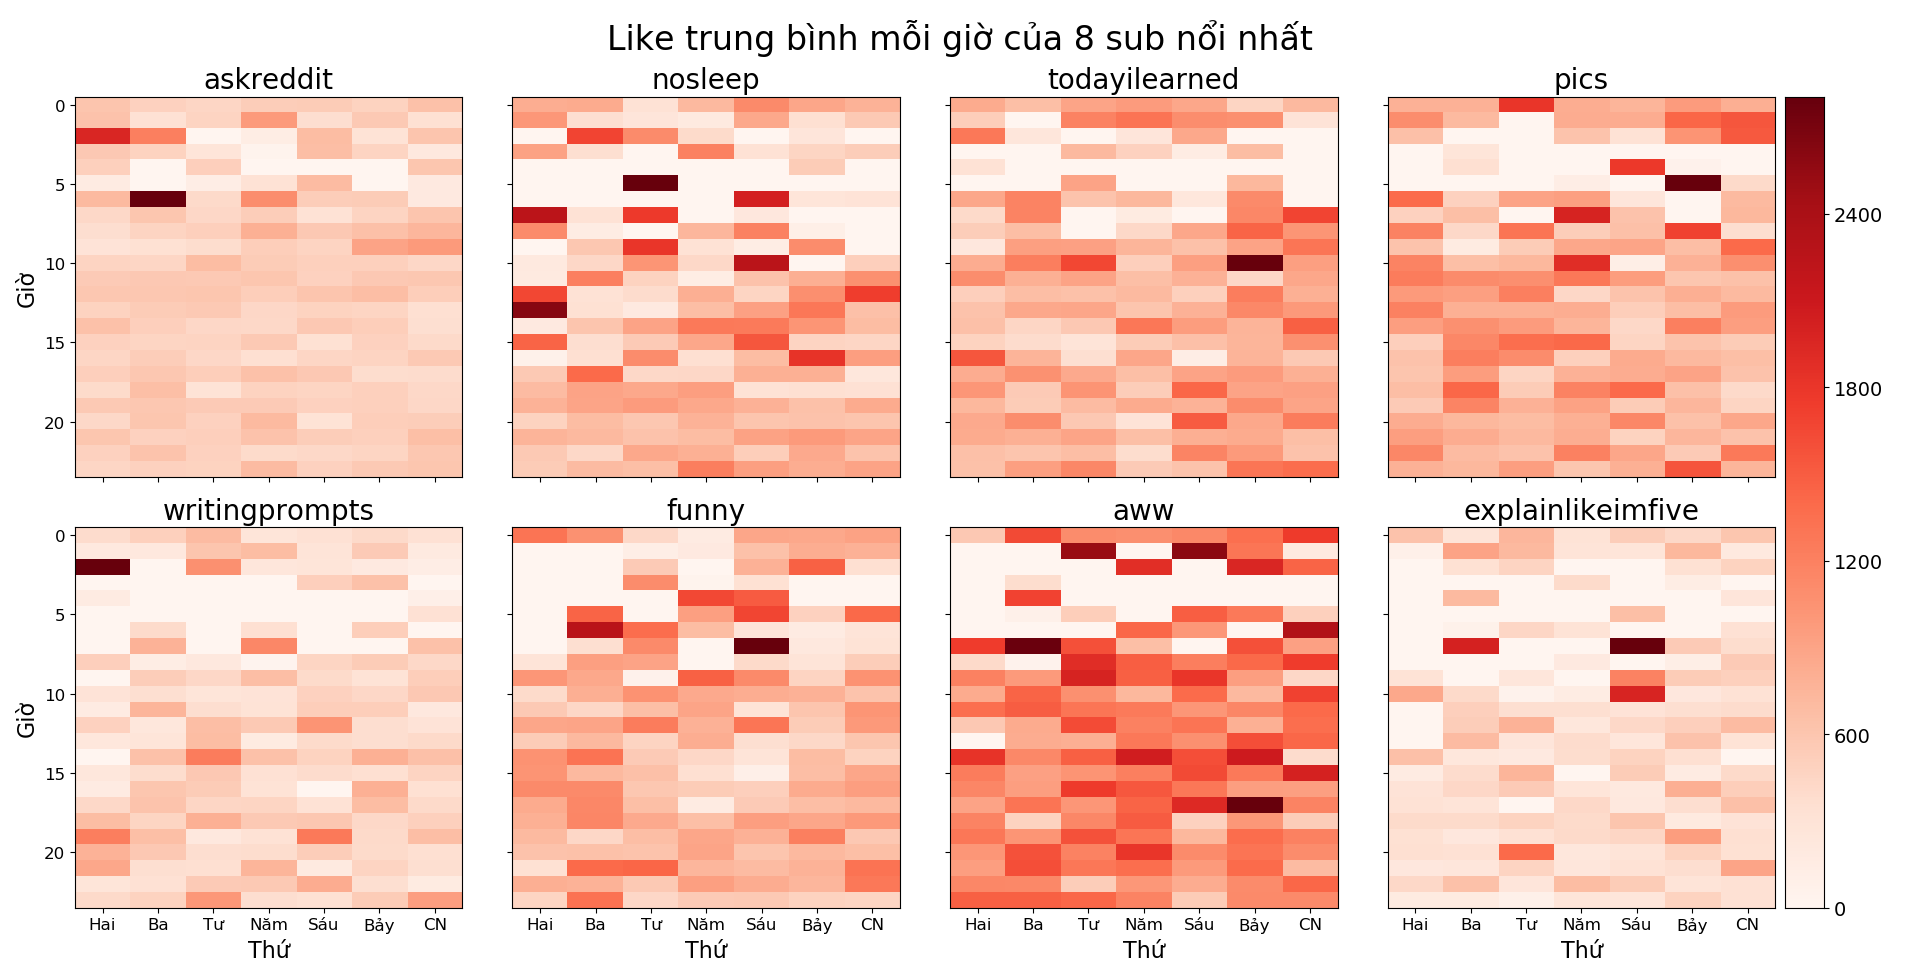
\includegraphics[width=\textwidth]{img/MeanLikesWeekdayHourPerSub.png}
    \caption{Like trung bình tính theo giờ đăng của 8 sub nổi nhất}
    \label{fig:meanlikesweekdayhourpersub}
\end{figure}

\textbf{askreddit} tuy có số like trung bình theo giờ thấp (dưới 800), song mức tương tác lại trải đồng đều ban ngày và ban đêm cả tuần, trừ hai trường hợp cá biệt 3 giờ sáng thứ hai và 6 giờ sáng thứ ba. Tức \textbf{askreddit} không hoàn toàn tuân theo xu hướng tổng thể (hình \eqref{fig:meanlikesweekdayhour}). Nhìn theo hướng khác, tương tác của \textbf{askreddit} là ổn định. Ngoài ra, \textbf{writingprompts} và \textbf{explainlikeimfive} cũng theo xu hướng tương tự.

Mặc dù \textbf{nosleep} thường xuyên được post vào ban đêm và có số like khá khẩm hơn \textbf{askreddit}, số phản ứng lại đến nhiều hơn với những bài đăng ban ngày vào ban ngày. Quy tắc không thể hiện rõ nhưng có vài điểm tập trung khác thường vào hai, tư và sáu. Phải chăng các độc giả sẽ ít sợ nút like vào ban ngày hơn?

Mỗi sub còn lại ít nhiều gì cũng có số like tương đồng bất kể giờ đăng. Riêng \textbf{pics}, \textbf{funny} và \textbf{aww} tiếp tục được nhận tương tác nhiều hơn các sub "tường chữ" một cách rõ rệt.

\section{Dịch giả RedditVN}
Cùng điểm một số số liệu thống kê về những chú kiến thợ của RedditVN.
\subsection{Thống kê tổng quát}
Tổng số dịch giả: 2458.

Mỗi dịch giả trung bình dịch 9 bài.

Dịch giả chăm chỉ nhất: Hoàng Anh Lâm, với 289 bài. Và bạn cũng là người được like nhiều nhất: 374356 like.

Địa chỉ Facebook: \href{https://facebook.com/100003092005874}{https://facebook.com/100003092005874}.

Xét bình quân, dịch giả được cưng yêu nhất: Phạm Bảo Hưng, với trung bình 5168 like mỗi bài. Dù thực ra, bạn chỉ dịch đúng một bài.

Địa chỉ Facebook: \href{https://facebook.com/100004271236056}{https://facebook.com/100004271236056}.

\begin{itemize}
    \item 498 dịch giả (20.26\%) có 10 bài dịch trở lên.
    \item 259 dịch giả (10.54\%) có 20 bài dịch trở lên.
    \item 97 dịch giả (3.95\%) có 50 bài dịch trở lên.
    \item 29 dịch giả (1.18\%) có 100 bài dịch trở lên.
    \item 6 dịch giả (0.24\%) có 200 bài dịch trở lên.
\end{itemize}

Có gần 80\% dịch giả có dưới 10 bài dịch nên mô hình thống kê là không cần thiết.

\subsection{Lựa chọn dịch bài}
Chúng ta cùng xem các dịch giả có xu hướng chọn bài như thế nào, dựa trên hai tiêu chí: độ nổi và độ cũ của submission gốc.

Ở đây, chúng ta giả sử mỗi dòng trong bảng dữ liệu chỉ dịch một submission. Tất nhiên vẫn có những bài tổng hợp vài submission nhưng rất hiếm. Thật vậy, trong 22869 bài, chỉ có 534 bài đính kèm 2 link Reddit trở lên, chiếm 2,34\%: không đáng kể.

Trước hết, tương tự các bài dịch tiếng việt ở trên, chúng ta phải kiểm tra tỉ số giữa karma và số bình luận trong một bài submission gốc.


\end{document}